\clearpage
\section{Processes}

\subsection{Scrum}
We implemented our project utilizing the Scrum framework.
Over the course of the project, we completed six \glspl{Sprint}\index{Sprint}.
Within these sprints, we tackled seven \glspl{Epic}\index{Epic}, and successfully completed a total of 54 User Stories.
The progression of our project, along with the milestones and deliverables achieved, is illustrated in the Gantt chart in Figure \ref{fig:scrum_gantt}.

\begin{figure}[h!]
	\center
	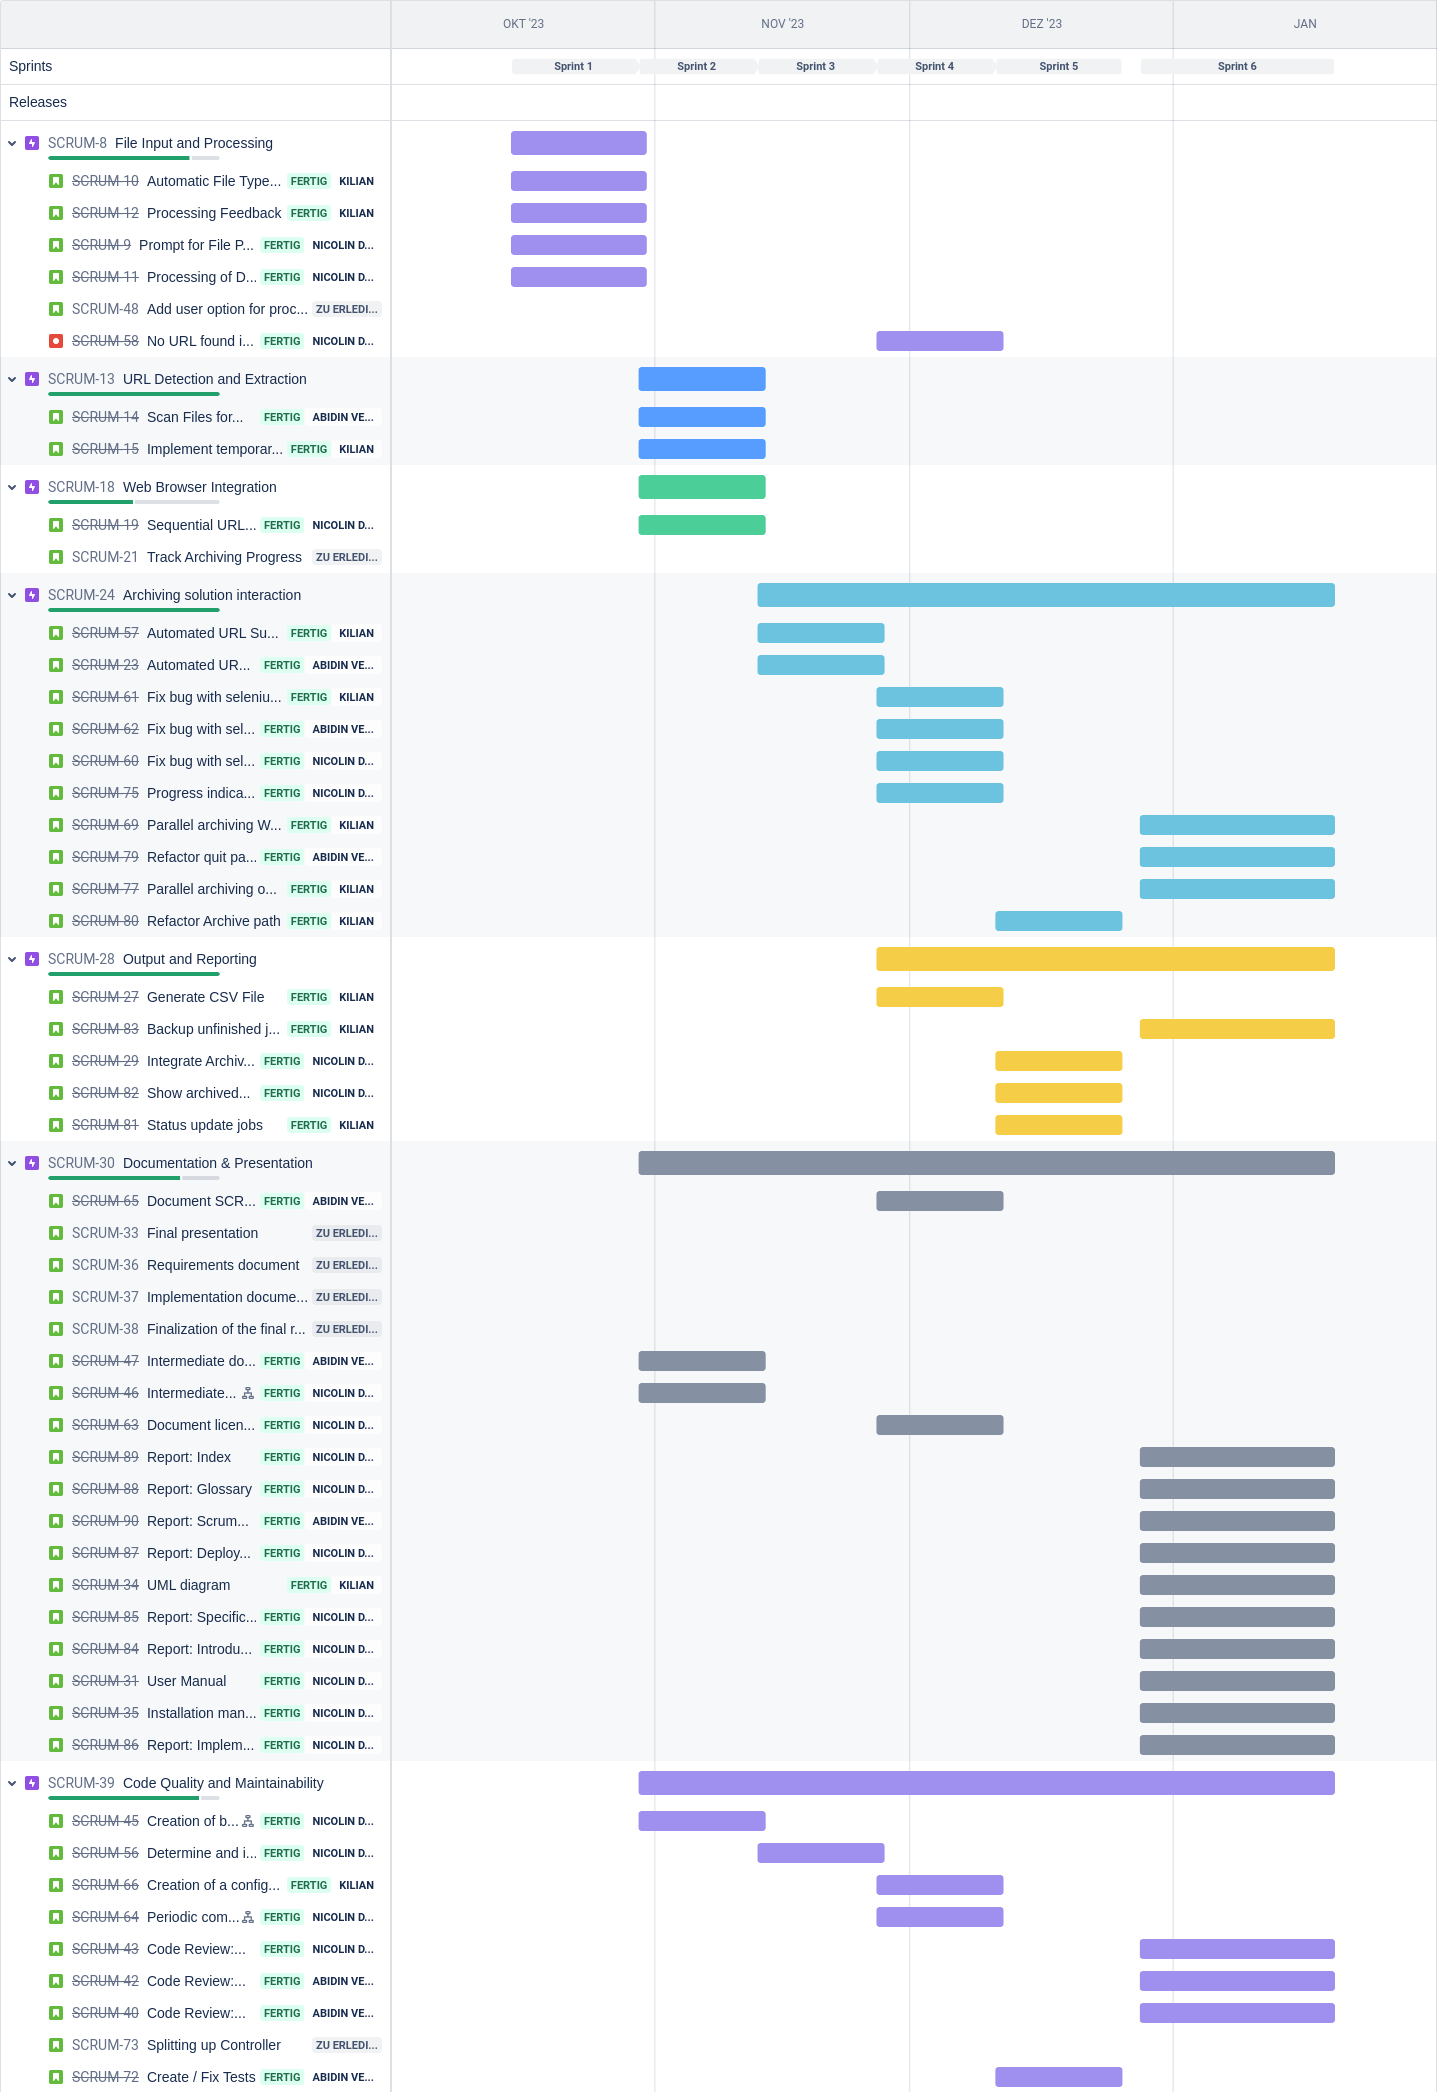
\includegraphics[width=0.99\textwidth]{pictures/Scrum/GANTT.png}
	\caption{Comprehensive GANTT Chart Overview of Sprint Timelines}
	\label{fig:scrum_gantt}
\end{figure}

\subsection{Allocation of roles}
In this chapter, the Scrum roles (Product Owner, Scrum Master, Developer) and additional roles such as Customer, Stakeholder, etc. are defined.


\subsection{Scrum roles}
We have decided to structure our Scrum team \index{Scrum team} in the following manner:
\begin{table}[ht]
    \centering
    \begin{bfhTabular}{lll}
        \textbf{Role} & \textbf{Person}\\\hline
        Product Owner & Nicolin Dora\\\hline
        Scrum Master  & Abidin Vejseli\\\hline
        Developer     & Nicolin Dora, Abidin Vejseli, Kilian Wampfler\\\hline
    \end{bfhTabular}
    \caption{Scrum Roles}
    \label{tab:tab1}
\end{table}

Nicolin took on the role of Product Owner \index{Product Owner} as he had concrete ideas and visions for the product at the start of the project.
Additionally, he took on this role because he wanted to deal with the subjects surrounding the product backlog.

Abidin took on the role of the Scrum Master \index{Scrum Master} as he has the most experience with the agile way of working.
He has already had the opportunity to perform this role professionally on several smaller projects in the past.

Kilian took on the role of a Developer \index{Developer}, as he is an active programmer in his job and has already gained some experience with Scrum.
Therefore, self-organization is not a foreign concept to him.

Besides Kilian, all the other members of the group were also assigned the role of Developer, as otherwise the project would not have been feasible in the given time. This is due to the fact that we all work alongside the university.

\subsection{Additional roles}
In addition to the Scrum roles, we have assigned the following roles to our specialist lecturer and PM-coach.
\begin{table}[ht]
    \centering
    \begin{bfhTabular}{lll}
        \textbf{Role} & \textbf{Person}\\\hline
        Stakeholder   & Dr. Simon Kramer\\\hline
        Customer      & Dr. Simon Kramer\\\hline
        PM-Advisor    & Frank Helbling\\\hline
    \end{bfhTabular}
    \caption{Additional Scrum Roles}
    \label{tab:tab2}
\end{table}

\subsection{Scrum Adaptionen}
As part of Project 1, we have adjusted Scrum in order to use it in the best possible way.
The major adjustments are explained in this chapter.

\subsubsection{Definition of Ready (DOR)}
Our DOR \index{Definition of Ready (DOR)} includes conditions that ensure that all team members understand the user stories and know when a \gls{UserStory} can be included in a sprint. The DOR was set in line with the INVEST\footnote{\href{https://xp123.com/articles/invest-in-good-stories-and-smart-tasks/}{XP123 article: Invest in good stories and smart tasks}} criteria. A user story in the product backlog must meet the DOR before it can be included in a sprint.

\textbf{Definition of Ready}
\begin{itemize}
    \item Ensure a clear definition
    \item Define the functionality or requirement to be implemented
    \item Clearly defined and testable acceptance criteria
    \item Ensure there are no or minimal dependencies
    \item Understood by the whole team
    \item The user story has been estimated
    \item The scope of the user story is small enough that it can be implemented in a single sprint.
\end{itemize}

\subsubsection{Definition of Done (DOD)}
Our DOD \index{Definition of Done (DOD)} contains all the characteristics and standards that a user story must meet to be considered complete.
Once it satisfies the necessary quality requirements (acceptance criteria), the story can be considered complete and can be closed.
The goal of our DOD is to create transparency so that everyone has a common understanding of when a story can be closed.
A story that does not comply with the DOD may not be finalised.

\textbf{Definition of Done}
\begin{itemize}
    \item Coding standards and best practices are implemented
    \item Unit tests for the feature are written and passe
    \item Any changes to the code or functionality are documented
    \item The code and functionality are reviewed by peers
    \item The feature works across multiple platforms
    \item Code is integrated with master branch
    \item Documentation has been updated
    \item Acceptance criteria are met
\end{itemize}

\subsubsection{Sprint}
As a team, we have decided that our sprints will take place at two-week intervals.
For each sprint we define a SMART sprint goal, which specifies the relevant user stories.

We decided in favour of the two-week rhythm because regular feedback is important to us and thus creates a greater learning effect.
Additionally, we ascertained that one-week sprints would result in excessive overheads due to the administrative work involved in Scrum.
Likewise, we consider sprints longer than two weeks to be impractical, as the interaction would suffer.

\subsubsection{Daily Scrum}
As a team, we have decided not to have daily Scrum meetings, as this is not possible because all team members do work part times. Instead, we have two weekly meetings (weeklys), on Wednesday and Friday at 17:00, which last a maximum of 15 minutes.
In addition, we have chosen to hold the meetings through Microsoft Teams as it is easier to organise.
The goal of these meetings is to share the current progress, address issues, update the team and briefly discuss the next steps.